\hypertarget{part-2-image-4}{%
	\section{Part 2, Image 4}\label{part-1-design-2}}

\centering


\hypertarget{description}{%
	\subsubsection{Description}\label{description}}

\begin{description}
	\item[Image:]
	\item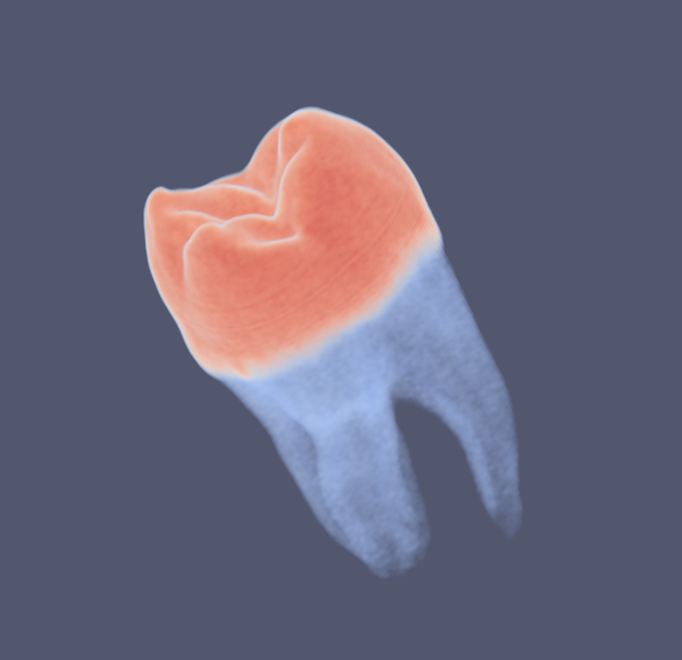
\includegraphics[width=9cm]{Tooth2.png}
	
	\item[Tool:]
	\hfill \break
		Paraview
	\item[Visual Mappings:]
	\begin{itemize}
		\tightlist
		\item[ ]
	\end{itemize}
	\begin{itemize}
		\tightlist
		\item
		\textbf{Mapping 1}: 
		\hfill \break
			The colour preset for the colour mapping is cool to warm. At data point 596.390 to 787.088, the opacity is 0.000, and this is assigned the darkest part of the blue. At 787.088 the opacity line goes up linearly to 100.000 at data point 1300.000, which has the deepest red value. At data point 948.195 is where the white colour value has been assigned.
	\end{itemize}
	
	\begin{itemize}
		\tightlist
		\item
		\textbf{Mapping 2}: 
		\hfill \break
			The colour space is set to diverging, and the nan opacity is set to 1. The colour discretion is set to a value of 256 number of table values.
	\end{itemize}
	\item[Data Conversion:] 
	\hfill \break
		Data scalar type unsigned short was used with a representation of volume used. Volume rendering was set to smart, and a blend mode of Composite is selected. Data extent: 0 - 511, 0 - 511, 0 - 181 was used and data byte order of BigEndian.
	\item[Unique Observation:]
	\hfill \break
		At datapoint 948.195 is where the transition from the root to the actual tooth. This is the white stripe in the image.
	
\end{description}